\documentclass[11pt]{book}
\usepackage{gvv-book}
\usepackage{gvv}
\usepackage[sectionbib,authoryear]{natbib}
\setcounter{secnumdepth}{3}
\setcounter{tocdepth}{2}
\makeindex

\begin{document}
\frontmatter
\tableofcontents
\setcounter{page}{0}
\mainmatter
\chapter{Triangle}
Consider a triangle with vertices
\begin{align}
\label{eq:tri-pts}
\vec{A}=\myvec{-3 \\ 0},\,
\vec{B}=\myvec{4\\2},\,
	\vec{c}=\myvec{1\\4},\,
\end{align}

\section{Vectors}
\section{Median}
\section{Altitude}

\begin{enumerate}[label=\thesection.\arabic*.,ref=\thesection.\theenumi]
\numberwithin{equation}{enumi}

%Question 1.3.1:
\item $\vec{D}_1$ is a point on $BC$ such that
\begin{align}
AD_1 \perp BC
\end{align}
and $AD_1$ is defined to be the altitude. Find the normal vector of $AD_1$.
  \\   \solution Given  \\
  \begin{align} 
 \vec{A} &= \myvec{ -3\\ 0 } \\
 \vec{B} &= \myvec{ 4\\ 2 }\\
 \vec{C} &= \myvec{ 1\\ 4}
 \end{align}
The normal vector of $AD_{1}$ is orthogonal to $AD_1$ and hence parallel to $BC$ \\ Direction vector $\vec{m_{BC}}$ 
\begin{align}
    &=\vec{C}-\vec{B}\\
    &=\myvec{1 \\ 4} -\myvec{4 \\2} \\
    m_{BC} &= \myvec{-3 \\ 2}
\end{align}
Normal vector of $AD_1$ is
\begin{align}
\label{eq:norm_vec_AD1}
	\vec{n} &= 
\myvec{-3\\2}
\end{align}

  %Question 1.3.2:
\item Find the equation of $AD_1$.
 \\    \solution from \eqref{eq:norm_vec_AD1} 
 \begin{align}
	\vec{n} &= 
\myvec{-3\\2}
\end{align}

The equation of $AD_1$ is
\begin{align}
 \vec{n}^{\top}(\vec{x-A}) &= 0 \\
\implies \myvec{-3 & 2}\vec{x} &= \myvec{-3& 2}\myvec{-3 \\ 0}\\
\myvec{-3 & 2}\vec{x} &= 9
\end{align}
see \figref{fig:line_ad}
\begin{figure}[H]
    \centering
    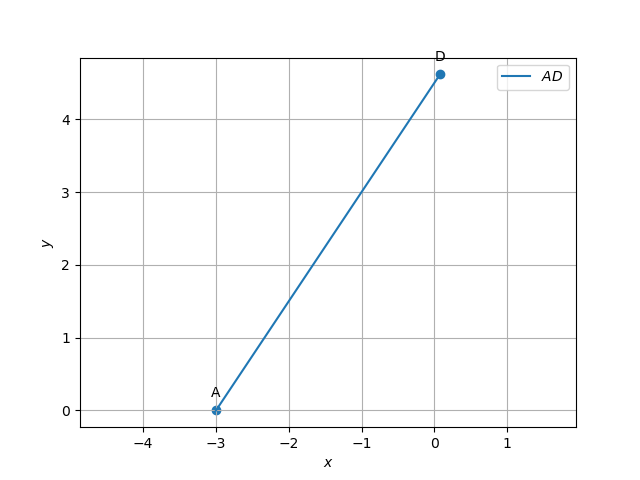
\includegraphics{/sdcard/geometry/geometry/figs/ramalt1.png}
    \caption{Line AD}
    \label{fig:line_ad}
\end{figure}
 
%Question 1.3.3:
\item Find the equations of the altitudes $BE_1$ and $CF_1$ to the sides $AC$ and $AB$ respectively. 
  \\    \\ \solution Given 
    \begin{align} 
 \vec{A} &= \myvec{ -3\\ 0 } \\ 
 \vec{B} &= \myvec{ 4\\ 2 }\\
 \vec{C} &= \myvec{ 1\\ 4}
 \end{align}
 Direction vector 
 \begin{align}
     \vec{m_{AB}}&=\vec{B}-\vec{A} \\
           &=\myvec{4 \\ 2} -\myvec{-3 \\ 0}  \\
           &=\myvec{7 \\2} \\
    \vec{ m_{AC}}&=\vec{C}-\vec{A} \\
     &=\myvec{1 \\ 4} -\myvec{-3 \\ 0}  \\
     &=\myvec{4 \\ 4} \\
 \end{align}
  Normal vector of $BE_1$ is orthogonal to $BE_1$  and hence parallel to $AC$ and normal vector of $CF_!$ is orthogonal to $CF_1$ and hence parallel to $AB$
  \begin{align}
      \vec{n_{BE_1}}&=\vec{m_{AC}}\\
      &=\myvec{4 \\ 4}\\
      \vec{n_{CF_1}}&=\vec{m_{AB}}\\
      &=\myvec{7 \\ 2}\\
  \end{align}
  Equation of line is represented by :
  \begin{align}
      \vec{n}^{\top}\myvec{\vec{x}-\vec{p}}&=0
  \end{align}
  \begin{enumerate}
      \item The equation of line $CF_1$
      \begin{align}
          \vec{n}^{\top}_{CF_1}\myvec{\vec{x}-\vec{C}}&=0 \\
          \vec{n}^{\top}{CF_1}\vec{x}&= \vec{n}^{\top}{CF_1}\vec{C} \\
          \myvec{7 \\2}^{\top}\vec{x}&=\myvec{7 \\ 2}^{\top}\myvec{1 \\ 4}\\
          \myvec{7 & 2}\vec{x}&=15
      \end{align}
      \item The equation of line $BE_1$
      \begin{align}
          \vec{n}^{\top}_{BE_1}\myvec{\vec{x}-\vec{B}}&=0 \\
          \vec{n}^{\top}{CF_1}\vec{x}&= \vec{n}^{\top}{BE_1}\vec{B} \\
          \myvec{4\\4}^{\top}\vec{x}&=\myvec{4 \\ 4}^{\top}\myvec{4 \\ 2}\\
          \myvec{4 & 4}\vec{x}&=2
      \end{align}
  \end{enumerate}
`
  

  %Question 1.3.4:
\item Find the intersection $\vec{H}$ of $BE_1$ and $CF_1$.
 \\  \solution Equation of $\vec{BE_1}$ \\
\begin{align}
    \myvec{7 & 2}\vec{x}&= 15
\end{align}
Equation of $\vec{CF_1}$ \\
\begin{align}
    \myvec{4 & 4}\vec{x}&=24
\end{align}
Therefore ,we need to solve the following equation to get $\vec{H}:$ \\
\begin{align}
        \myvec{7&2\\4&4} \vec{x} &= \myvec{15\\24}
\end{align}
%
which can be solved as 
%
yielding
%
\begin{align}
        \vec{H}&=\myvec{{\frac{3}{5}}\\ \frac{27}{5}}
		\label{eq:geo-alt-H},
\end{align}
%
See 
\figref{fig:m_tri_py}
\begin{figure}[H]
\centering
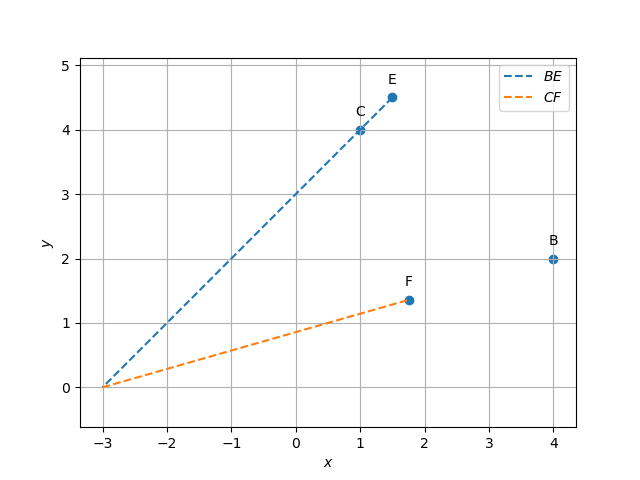
\includegraphics[width=\columnwidth]{/sdcard/geometry/geometry/figs/ramalt2.png}
\caption{Intersection point $\vec{H}$ of altitudes B$E_{1}$ and C$F_{1}$ plotted using python}
\label{fig:m_tri_py}
\end{figure}

 %Question 1.3.5:
\item Verify that 
		\begin{align}
			\brak{\vec{A}-\vec{H}}^{\top}\brak{\vec{B}-\vec{C}} = 0
		\end{align}
\\  \solution
 \begin{align} 
 \vec{A} &= \myvec{ -3\\ 0 } \\ 
 \vec{B} &= \myvec{ 4\\ 2 }
  \\\vec{C} &= \myvec{ 1\\ 4} \\ 
  \vec{H} &=\myvec{\frac{3}{5}\\ \frac{27}{5}}
 \end{align}
\begin{align}
\vec{A}-\vec{H}=\myvec{\frac{-18}{5}\\ \frac{-27}{5}},\,
\vec{B}-\vec{C}=\myvec{3\\-2}
\\
	\implies \brak{\vec{A}-\vec{H}}^{\top}\brak{\vec{B}-\vec{C}}=\myvec{\frac{-18}{5} & \frac{-27}{5}}
\myvec{3\\-2}
=0
\end{align}
see \figref{fig:Pts_ABCH}
\begin{figure}
    \centering
    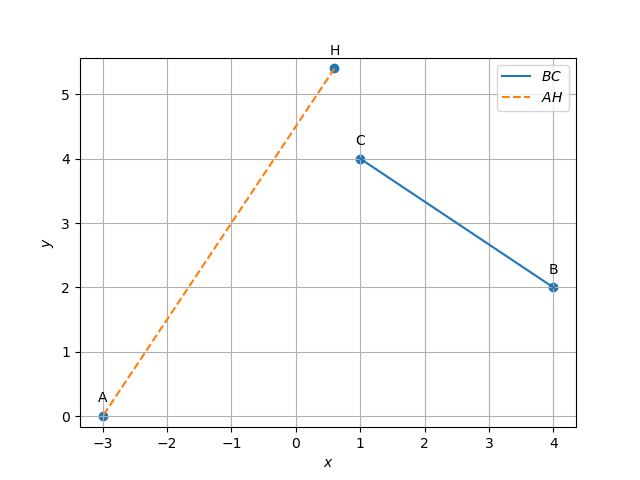
\includegraphics{/sdcard/geometry/geometry/figs/ramalt3.png}
    \caption{Plot of points A,B,C and H}
    \label{fig:Pts_ABCH}
\end{figure}



\end{enumerate}
\end{document} 
